\documentclass[a4paper,11pt]{article}
\pdfoutput=1 % if your are submitting a pdflatex (i.e. if you have
             % images in pdf, png or jpg format)

\usepackage{jheppub} % for details on the use of the package, please
                     % see the JHEP-author-manual
\usepackage{cleveref}
\usepackage{float}
\usepackage{booktabs} % For professional quality tables (\toprule, \midrule, \bottomrule)
\usepackage{array}    % For table column formatting (p{} columns)
\usepackage{caption}  % For table captions
\usepackage{pdflscape} % *** ADDED THIS LINE TO FIX THE 'landscape' ENVIRONMENT ERROR ***
\usepackage{graphicx}
\usepackage{tabularx}
\usepackage[T1]{fontenc} % if needed



\title{\boldmath Primordial Cosmological Perturbations under Invertible Higher-Derivative Disformal Transformation and other Disformal Transformations}


%% %simple case: 2 authors, same institution
%% \author{A. Uthor}
%% \author{and A. Nother Author}
%% \affiliation{Institution,\\Address, Country}

% more complex case: 4 authors, 3 institutions, 2 footnotes
\author[1]{Allan L. Alinea,\note{Corresponding author.}} 
\author[]{John Onesimus G. Ancheta}


\affiliation[]{Astrophysics, Particle Physics, Nuclear Physics Research Cluster
\\Institute of Physics, \\ University of the Philippines Los Baños \\ 4031 College, Los Baños, Laguna, Philippines}

% e-mail addresses: one for each author, in the same order as the authors
\emailAdd{alalinea@up.edu.ph}
\emailAdd{jgancheta@up.edu.ph}





\abstract{
Primordial comsmological perturbations are quantum fluctuations that served as seeds in the early universe
for what we nowadays observe as galaxies and clusters thereof. Cosmic inflation and the accompanying dynamics
of the expanding Universe, stretched and allowed them to evolve, leading to their current state. 
Being the "beginning" of us all, their importance cannot be overemphasised. 
Focusing on their mathematical properties, in this study, we explore their possible variation under different forms of disformal transformation.
This goes from reviews for the simplest special disformal transformal, passing through the original Bekenstein disformal transformation, 
and then leading to investigation of the effect of the Invertible Higher-Derivative Disformal Transformation (TMM disformal transformation). 
We examine the variations of scalar and tensor perturbations within the framework of the Horndeski theory. 
While footprints of the change of these perturbations may be apparent at the leading order, we find that the stretching of the early universe may remove these marks of variance in the superhorizon limit.
\note{what in the world}
}



\begin{document} 
\maketitle
\flushbottom

\section{The purpose of this document} \label{sec:purpose}
Although this document is currently formatted in the style of JHEP, it is not yet meant
to be a submission to JHEP or any journal thereof. This document, serves as two things. Firstly, it is where the second author
fleshes out his thoughts regarding the topic, and thus the calculations and discussions may be lengthy and verbose.
The second author wishes to grasp and understand the topics at hand. Secondly, it serves as a template and source material
for a future formal document that may be submitted to JHEP or any other journal; it might even be a springboard for the author's undergraduate thesis. 


\section{Overview and thoughts}


\section{Mathematical Preliminaries} 


\subsection{The Riemann Curvature Tensor and its Contractions}
\label{subsec:RCT}
 A \textbf{manifold} is a topological space that is locally Euclidian. On the other hand a \textbf{Riemannian manifold} is a type of 
 manifold where mesaurement of distance and angle is possible. This is made possible by the metric. 

 An aside. Gauss figured out that any point on a 2D surface can be summarized by a single number which
 we denote as $K$ and is called as the \textbf{Gaussian curvature}. This is the product of the two principal curvatures
 at a particular point. Simply put, the principal curvatures are rough approximations of the 2D surface.
\begin{figure}[H]
\centering
\def\imgwidth{0.65\linewidth}
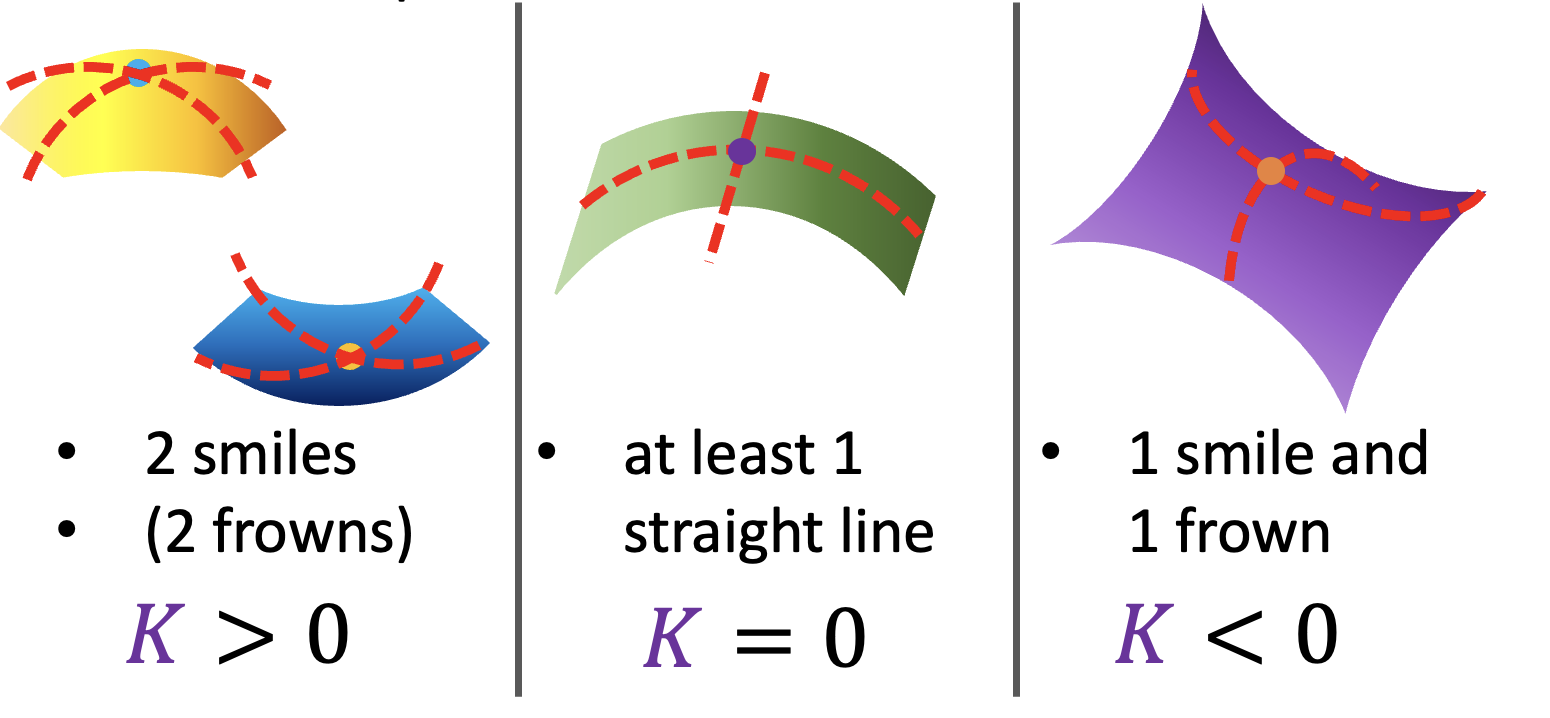
\includegraphics[width=\imgwidth]{pasted-images/primordial-cosmological-perturbations-00-21-20.png}
\caption{According to Gaussian Curvature, if you have a surface that can be approximated
by two “frowns” or “smiles”, then the intersection thereof has positive curvature ($K>0$).
If one is a “frown” and the other a “smile”, the intersection has negative curvature ($K<0$).
If one direction is flat, the curvature is zero ($K=0$).}
\label{fig:gaussian-curvature}
\end{figure}
The issue with the Gaussian Curvate is that it only works for 2D surfaces. This motivates
us to develop something that can work for higher dimensions. This is where we use the \textbf{Riemann Curvature Tensor} (RCT) given by
\begin{equation}
    R^\rho_{\ \sigma\mu\nu} = \partial_\mu \Gamma^\rho_{\nu\sigma} - \partial_\nu \Gamma^\rho_{\mu\sigma} + \Gamma^\rho_{\mu\lambda} \Gamma^\lambda_{\nu\sigma} - \Gamma^\rho_{\nu\lambda} \Gamma^\lambda_{\mu\sigma}.
    \label{riemann-curvature-tensor}
\end{equation}

Although we say that the Christofell Symbols are non-tensorial in nature, the 
sum thereof ammounting to the Riemann Curvature Tensor is indeed a tensor. 
We can think of the Christofell Symbols as mathematical objects that describe how the 
coordinate basis vectors change from point to point on a given manifold. Note that
the covariant derivative (which is related to the original definition of the RCT) is related
to the Christofell Symbols as follows:

\begin{equation}
    \nabla_\mu V^\rho = \partial_\mu V^\rho + \Gamma^\rho_{\mu\sigma} V^\sigma.
    \label{covariant-derivative-christofell}
\end{equation}



\section{History and Properties of the Universe}
The Universe as we see it today is \textbf{homogenous} and \textbf{isotropic}. Homogeneity talks about

\subsection{What the Cosmic Microwave Background Tells us}
For the first $\sim400,000$ years of the Universe, it was too hot to allow atoms to form, at
this stage electrons have yet to couple with protons. Due to quantum mechanical effects, free electrons scatter
the photons of the early univers, making it opaque, thereby "trapping" the photons. 
However, as the Universe expanded and cooled, it eventually reached a temperature
where electrons could finally couple with protons to form atoms. At this point,
photons could finally travel freely through space. This photons, given the extreme nature of the early universe
were highly energetic, and so we must be careful in observing them today.

The continuous expansion of the universe
stretched the photons, thereby increasing their wavelength. If we traceback this stretching from the time when 
photons started to propagate freely up to the present time, we find these photons fall in the microwave region. 
This is what we now call as the Cosmic Microwave Background (CMB). It is a strong evidence that, indeed, 
the universe started from a hot and dense state, and has been expanding ever since. 







\section{The Expanding and Flat Universe}
The FLRW metric is given by 
\begin{equation}
    ds^2 = -dt^2 + a^2(t) \left[ \frac{dr^2}{1-Kr^2} + r^2 (d\theta^2 + \sin^2 \theta d\phi^2) \right],
    \label{flrw-metric}
\end{equation}





As discussed in \ref{subsec:RCT} a Gaussian Curvature of $K=0$ denotes a flat space. Would it make sense
to probe perturbations in a flat universe? Observations show (take for example the CMB), indicate
that our universe is close to being spatially flat. We can actually study the perturbations by 
looking into the deviations from a flat, homogenous, and isotropic "background". Hence in this exposition,
we will consider the case where we have a flat universe, i.e., $K=0$ in \cref{flrw-metric}.



\subsection{An Example in using the FLRW Metric}

Consider a spatially flat Friedmann–Lemaître–Robertson–Walker (FLRW) metric with $c$ explicit,
$$ \mathrm{d}s^2 = -c^2\mathrm{d}t^2 + a(t)^2\bigl(\mathrm{d}r^2 + r^2\mathrm{d}\Omega^2\bigr). $$
A light signal emitted at cosmic time $t_{\rm em}$ from radial coordinate $r_{\rm em}$ and received at $t_0$ (so $r_{\rm obs}=0$) follows a radial null geodesic with $\mathrm{d}r = -c\,\mathrm{d}t/a(t)$. The comoving radial distance from observer to source is
$$ \chi \equiv r_{\rm em} = c\int_{t_{\rm em}}^{t_0}\frac{\mathrm{d}t}{a(t)}. $$
Assume the scale factor is a power law $a(t)=a_0\bigl(t/t_0\bigr)^n$ with $n\neq 1$.

\vspace{1em} % Adds a little vertical space
\begin{enumerate}
    \item Derive expressions for the comoving distance $\chi$, the proper distance today $D_{p}(t_0)$, the particle horizon, the luminosity distance $D_L$, and the angular diameter distance $D_A$.
    
    \item Then compute numerical values for these quantities for the matter-dominated case $n=\tfrac{2}{3}$ and redshift $z=1$.
    
    \item For the numerical example, use the normalization $a_0=1$, the relation $H_0=n/t_0$, and a Hubble constant of $H_0=70\ \mathrm{km\,s^{-1}\,Mpc^{-1}}$.
\end{enumerate}

\underline{\textbf{Solution:}}

\vspace{1em}

\textbf{Deriving $\chi$ for the travelling light}

Note for a travelling light we have a null geodesic, hence $ds^2=0$. 
Furthermore, since we have a travelling light in the radial direction,
there are no changes in the angular coordinates; in other words, $d\Omega^2 = 0$. 
Hence the FLRW metric reduces to
\begin{equation}
    0 = -c^2 dt^2 + a(t)^2 dr^2
    \label{null-geodesic-flrw}
\end{equation}

If we move the first term to the right and take the square root of both sides (taking note of the $\pm$)
then continuing to solve the differential equation, we have

\begin{align}
     cdt &= \pm a(t) dr\\
     dr &= \pm \frac{c}{a(t)} dt\\
     \chi &= \pm c \int_{t_0}^{t_{em}} \frac{1}{a(t)} dt
\end{align}

\begin{figure}[H]
\centering
\def\imgwidth{0.65\linewidth}
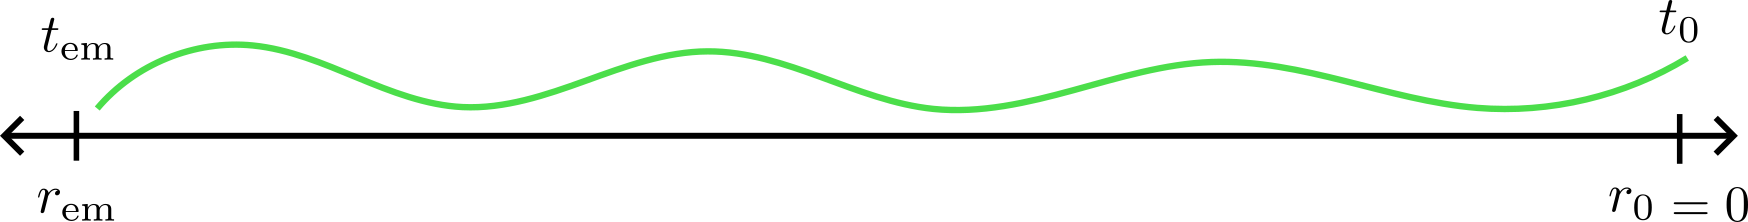
\includegraphics[width=\imgwidth]{pasted-images/comovinglight.png}
\caption{A light signal emitted at cosmic time $t_{\rm em}$ from radial coordinate $r_{\rm em}$ and received at $t_0$.}
\label{fig:comovinglight}
\end{figure}


If we refer to Fig. \ref{fig:comovinglight}, since as far as we know, time moves in one direction
then $dt>0$. On the other hand, notice that since we set $r_0=0$ as the obesrver's position,
as the light travel from $r_{em}$ to the observer, the distance decreases -- impying that $dr<0$.
It is now clear that in order to satifsy both conditions, we take the negative solution.

\begin{equation}
    \chi = -c \int_{t_0}^{t_{em}} \frac{1}{a(t)} dt
    \label{comoving-distance-integral}
\end{equation}

Does Eq. (\ref{comoving-distance-integral}) make sense? In my first encounter of this problem I was 
quite confused how this measures the comoving distance. Isn't the comoving distance supposed to be 
the "fixed" value prior to expansion at $t=t_{em}$? B



\section{Disformal Transformation}
\newpage
\begin{table}[H]
\centering
\caption{Types of Disformal Transformations of the Metric}
\label{tab:disformal}
\small
\renewcommand{\arraystretch}{1.9}

\begin{tabularx}{\textwidth}{@{} p{4.3cm} p{5.8cm} X @{}}
\toprule
\textbf{Transformation Name} & \textbf{Metric Transformation ($\hat{g}_{\mu \nu}$)} & \textbf{Short Description} \\
\midrule

Bekenstein &
$\hat{g}_{\mu \nu} = A(\phi)g_{\mu \nu} + B(\phi)\phi_{;\mu}\phi_{;\nu}$ &
The original proposal where both the conformal factor $A$ and disformal factor $B$ depend only on the scalar field $\phi$. \\

Special &
$\hat{g}_{\mu \nu} = g_{\mu \nu} + B(\phi, X)\phi_{;\mu}\phi_{;\nu}$ &
A purely disformal transformation with $A=1$. The disformal factor $B$ depends on $\phi$ and its kinetic term $X$. \\

Generalized with one arbitrary conformal &
$\hat{g}_{\mu \nu} = A(\phi)g_{\mu \nu} + B(\phi, X)\phi_{;\mu}\phi_{;\nu}$ &
A generalization where $A$ depends only on $\phi$, but $B$ depends on both $\phi$ and $X$. \\

Fully Generalized for First Derivatives &
$\hat{g}_{\mu \nu} = A(\phi, X)g_{\mu \nu} + B(\phi, X)\phi_{;\mu}\phi_{;\nu}$ &
Both the conformal factor $A$ and the disformal factor $B$ are allowed to depend on $\phi$ and its kinetic term $X$. \\

Fully General and Extended &
$\begin{array}[t]{@{}l@{}}
\hat{g}_{\mu \nu} = A(\dots)g_{\mu \nu} \\ + (C(\dots)\phi_{;\mu} + D(\dots)X_{;\mu}) \\
\hspace*{2em} \times (C(\dots)\phi_{;\nu} + D(\dots)X_{;\nu})
\end{array}$ &
The conformal factor $A$ and functions $C, D$ depend on $\phi$ and its invariants. The disformal part is a quadratic form involving gradients of $\phi$ and $X$. \\

TMM &
$\begin{array}[t]{@{}l@{}}
\hat{g}_{\mu \nu} = A(\dots) g_{\mu \nu} + B(\dots)\phi_{;\mu}\phi_{;\nu} \\
\quad + C(\dots)(\phi_{;\mu}X_{;\nu}+X_{;\mu}\phi_{;\nu}) \\
\quad + D(\dots)X_{;\mu}X_{;\nu}
\end{array}$ &
The most general quadratic transformation in first derivatives. All coefficient functions ($A, B, C, D$) depend on $\phi$ and its invariants ($X, Y, Z$). \\

\bottomrule
\end{tabularx}

\vspace{1em}
\footnotesize
\textbf{Note:} $X = -\frac{1}{2}g^{\alpha\beta}\phi_{;\alpha}\phi_{;\beta}$ denotes the kinetic term. The arguments $(\dots)$ in the last two rows are shorthand for $(\phi, X, Y, Z)$, representing dependence on the scalar field and its invariants.
\end{table}


\appendix
\section{Appendix} 
Please always give a title also for appendices.








\acknowledgments

This is the most common positions for acknowledgments. A macro is
available to maintain the same layout and spelling of the heading.

\paragraph{Note added.} This is also a good position for notes added
after the paper has been written.


haha



% The bibliography will probably be heavily edited during typesetting.
% We'll parse it and, using the arxiv number or the journal data, will
% query inspire, trying to verify the data (this will probalby spot
% eventual typos) and retrive the document DOI and eventual errata.
% We however suggest to always provide author, title and journal data:
% in short all the informations that clearly identify a document.

\begin{thebibliography}{99}

\bibitem{a}
Author, \emph{Title}, \emph{J. Abbrev.} {\bf vol} (year) pg.

\bibitem{b}
Author, \emph{Title},
arxiv:1234.5678.

\bibitem{c}
Author, \emph{Title},
Publisher (year).





\end{thebibliography}
\end{document}
